\documentclass[tikz,dvipdfmx,dvipsnames]{standalone}

\usepackage{amsmath, amssymb, amsthm, mathrsfs, amsfonts, dsfont}
\usepackage{bbm}
\usepackage{bm}
\usepackage{physics}
\usepackage{ifthen}
\usepackage{setspace}
\usepackage{mathtools}

\newcommand{\defeq}{\coloneqq}

\newcommand{\red}[1]{\textcolor{red}{#1}}
\newcommand{\blue}[1]{\textcolor{blue}{#1}}
\newcommand{\cyan}[1]{\textcolor{cyan}{#1}}
\newcommand{\gray}[1]{\textcolor{gray}{#1}}
\newcommand{\green}[1]{\textcolor{green}{#1}}
\newcommand{\brown}[1]{\textcolor{brown}{#1}}
\newcommand{\black}[1]{\textcolor{black}{#1}}
\newcommand{\orange}[1]{\textcolor{orange}{#1}}
\newcommand{\purple}[1]{\textcolor{purple}{#1}}
\newcommand{\yellow}[1]{\textcolor{yellow}{#1}}
\newcommand{\Magenta}[1]{\textcolor{Magenta}{#1}}
\newcommand{\RoyalBlue}[1]{\textcolor{RoyalBlue}{#1}}
\newcommand{\RubineRed}[1]{\textcolor{RubineRed}{#1}}
\newcommand{\ForestGreen}[1]{\textcolor{ForestGreen}{#1}}
\newcommand{\YellowOrange}[1]{\textcolor{YellowOrange}{#1}}
\newcommand{\WildStrawberry}[1]{\textcolor{WildStrawberry}{#1}}

\usetikzlibrary{calc,matrix,math}
\usetikzlibrary{decorations.pathreplacing,calligraphy}


\begin{document}
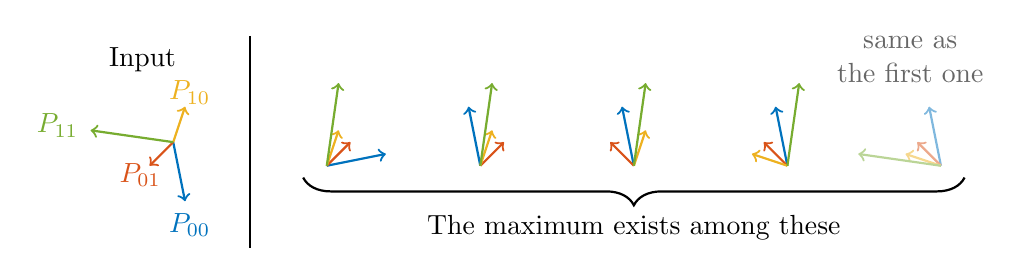
\begin{tikzpicture}[scale=0.15]
    \definecolor{cA}{HTML}{0072BD}
    \definecolor{cB}{HTML}{D95319}
    \definecolor{cC}{HTML}{EDB120}
    \definecolor{cD}{HTML}{77AC30}

    \node[anchor=center] at (13*-0.2,9) {Input};

    \foreach \x/\y/\ar/\ai/\br/\bi/\cr/\ci/\dr/\di/\alpha in {
            0/2/1/-5/-2/-2/1/3/-7/1/100,
            1/0/5/1/2/2/1/3/1/7/100,
            2/0/-1/5/2/2/1/3/1/7/100,
            3/0/-1/5/-2/2/1/3/1/7/100,
            4/0/-1/5/-2/2/-3/1/1/7/100,
            5/0/-1/5/-2/2/-3/1/-7/1/50
        }{
            \ifthenelse{\x=0}{
                \begin{scope}[yshift=\y cm]
                    \node[anchor=center,cA!\alpha] at (\ar*1.4,\ai*1.4) {$P_{00}$};
                    \node[anchor=center,cB!\alpha] at (\br*1.4,\bi*1.4) {$P_{01}$};
                    \node[anchor=center,cC!\alpha] at (\cr*1.4,\ci*1.4) {$P_{10}$};
                    \node[anchor=center,cD!\alpha] at (\dr*1.4,\di*1.4) {$P_{11}$};
                \end{scope}
            }{}
            \begin{scope}[xshift=13*\x cm, yshift=\y cm]
                \draw[->,thick,cA!\alpha] (0,0) -- (\ar,\ai);
                \draw[->,thick,cB!\alpha] (0,0) -- (\br,\bi);
                \draw[->,thick,cC!\alpha] (0,0) -- (\cr,\ci);
                \draw[->,thick,cD!\alpha] (0,0) -- (\dr,\di);
            \end{scope}
        }

    \node[black!60,anchor=center,align=center] at (13*4.8,9) {same as\\the first one};
    \draw (13/2,+11) -- (13/2,-7);
    \draw [
        thick,
        decoration={brace,mirror,amplitude=10pt},
        decorate
    ] (13-2,-1) -- (13*5+2,-1) node [pos=0.5,anchor=north,yshift=-10pt]
    {The maximum exists among these};
\end{tikzpicture}
\end{document}
